% Created by tikzDevice version 0.8.1 on 2015-05-24 13:12:09
% !TEX encoding = UTF-8 Unicode
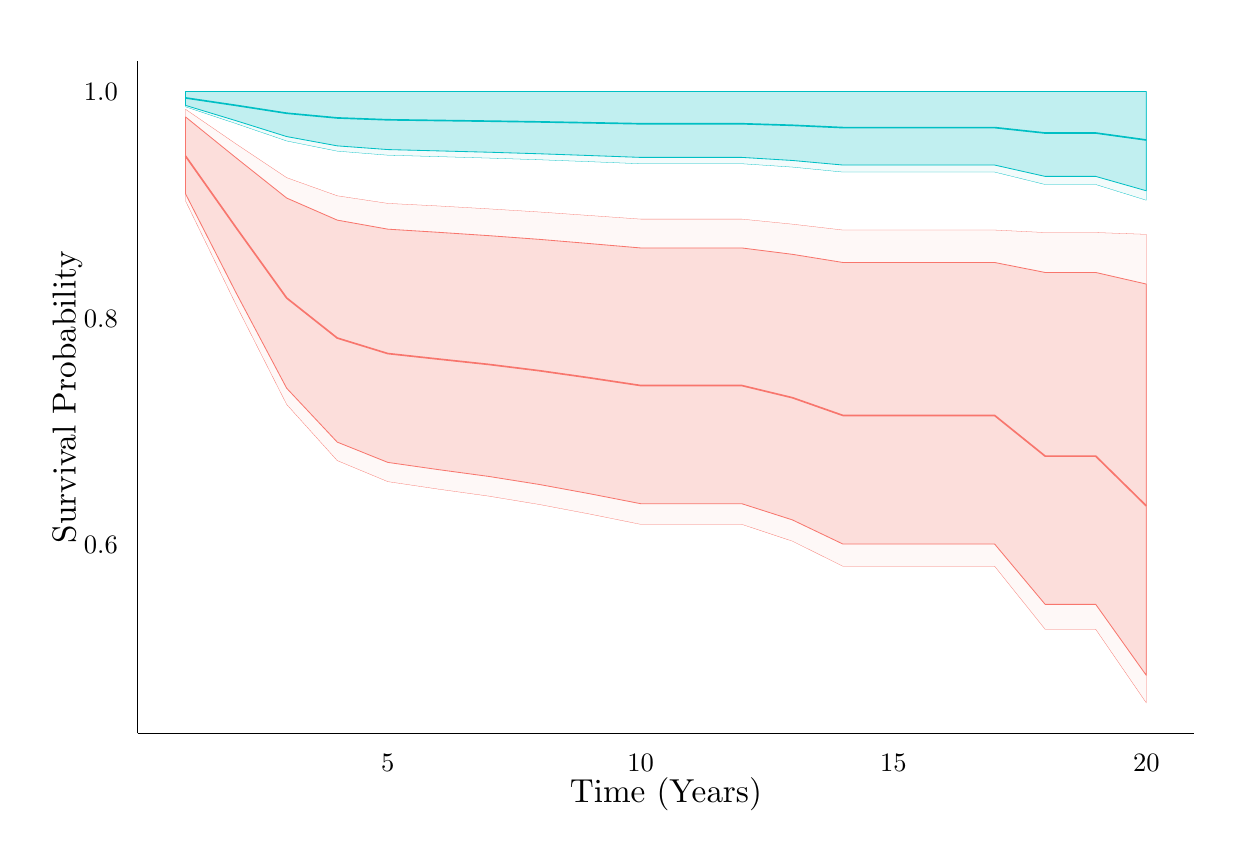
\begin{tikzpicture}[x=1pt,y=1pt]
\definecolor{fillColor}{RGB}{255,255,255}
\path[use as bounding box,fill=fillColor,fill opacity=0.00] (0,0) rectangle (433.62,289.08);
\begin{scope}
\path[clip] (  0.00,  0.00) rectangle (433.62,289.08);
\definecolor{drawColor}{RGB}{255,255,255}
\definecolor{fillColor}{RGB}{255,255,255}

\path[draw=drawColor,line width= 0.6pt,line join=round,line cap=round,fill=fillColor] (  0.00,  0.00) rectangle (433.62,289.08);
\end{scope}
\begin{scope}
\path[clip] ( 39.69, 34.03) rectangle (421.57,277.03);
\definecolor{fillColor}{RGB}{255,255,255}

\path[fill=fillColor] ( 39.69, 34.03) rectangle (421.58,277.03);
\definecolor{drawColor}{RGB}{248,118,109}

\path[draw=drawColor,line width= 0.6pt,line join=round] ( 57.05,242.67) --
	( 75.32,216.81) --
	( 93.59,191.39) --
	(111.86,176.93) --
	(130.13,171.32) --
	(148.41,169.33) --
	(166.68,167.38) --
	(184.95,165.12) --
	(203.22,162.52) --
	(221.49,159.77) --
	(239.77,159.77) --
	(258.04,159.77) --
	(276.31,155.37) --
	(294.58,148.96) --
	(312.86,148.96) --
	(331.13,148.96) --
	(349.40,148.96) --
	(367.67,134.25) --
	(385.94,134.25) --
	(404.22,116.27);
\definecolor{drawColor}{RGB}{0,191,196}

\path[draw=drawColor,line width= 0.6pt,line join=round] ( 57.05,263.69) --
	( 75.32,260.99) --
	( 93.59,258.16) --
	(111.86,256.46) --
	(130.13,255.79) --
	(148.41,255.54) --
	(166.68,255.30) --
	(184.95,255.03) --
	(203.22,254.70) --
	(221.49,254.36) --
	(239.77,254.36) --
	(258.04,254.36) --
	(276.31,253.80) --
	(294.58,252.97) --
	(312.86,252.97) --
	(331.13,252.97) --
	(349.40,252.97) --
	(367.67,251.01) --
	(385.94,251.01) --
	(404.22,248.49);
\definecolor{drawColor}{RGB}{248,118,109}
\definecolor{fillColor}{RGB}{248,118,109}

\path[draw=drawColor,line width= 0.1pt,line join=round,line cap=round,fill=fillColor,fill opacity=0.05] ( 57.05,259.58) --
	( 75.32,247.06) --
	( 93.59,234.87) --
	(111.86,228.33) --
	(130.13,225.58) --
	(148.41,224.65) --
	(166.68,223.60) --
	(184.95,222.47) --
	(203.22,221.19) --
	(221.49,219.90) --
	(239.77,219.90) --
	(258.04,219.90) --
	(276.31,218.08) --
	(294.58,215.95) --
	(312.86,215.95) --
	(331.13,215.95) --
	(349.40,215.95) --
	(367.67,215.05) --
	(385.94,215.05) --
	(404.22,214.40) --
	(404.22, 45.08) --
	(385.94, 71.67) --
	(367.67, 71.67) --
	(349.40, 94.47) --
	(331.13, 94.47) --
	(312.86, 94.47) --
	(294.58, 94.47) --
	(276.31,103.54) --
	(258.04,109.61) --
	(239.77,109.61) --
	(221.49,109.61) --
	(203.22,113.30) --
	(184.95,116.77) --
	(166.68,119.79) --
	(148.41,122.33) --
	(130.13,125.04) --
	(111.86,132.64) --
	( 93.59,152.92) --
	( 75.32,188.90) --
	( 57.05,226.46) --
	cycle;
\definecolor{drawColor}{RGB}{0,191,196}
\definecolor{fillColor}{RGB}{0,191,196}

\path[draw=drawColor,line width= 0.1pt,line join=round,line cap=round,fill=fillColor,fill opacity=0.05] ( 57.05,265.99) --
	( 75.32,265.99) --
	( 93.59,265.99) --
	(111.86,265.99) --
	(130.13,265.99) --
	(148.41,265.99) --
	(166.68,265.99) --
	(184.95,265.99) --
	(203.22,265.99) --
	(221.49,265.99) --
	(239.77,265.99) --
	(258.04,265.99) --
	(276.31,265.99) --
	(294.58,265.99) --
	(312.86,265.99) --
	(331.13,265.99) --
	(349.40,265.99) --
	(367.67,265.99) --
	(385.94,265.99) --
	(404.22,265.99) --
	(404.22,226.72) --
	(385.94,232.40) --
	(367.67,232.40) --
	(349.40,236.90) --
	(331.13,236.90) --
	(312.86,236.90) --
	(294.58,236.90) --
	(276.31,238.70) --
	(258.04,239.91) --
	(239.77,239.91) --
	(221.49,239.91) --
	(203.22,240.65) --
	(184.95,241.35) --
	(166.68,241.95) --
	(148.41,242.48) --
	(130.13,243.00) --
	(111.86,244.46) --
	( 93.59,248.14) --
	( 75.32,254.40) --
	( 57.05,260.47) --
	cycle;
\definecolor{drawColor}{RGB}{248,118,109}
\definecolor{fillColor}{RGB}{248,118,109}

\path[draw=drawColor,line width= 0.3pt,line join=round,line cap=round,fill=fillColor,fill opacity=0.20] ( 57.05,256.82) --
	( 75.32,242.03) --
	( 93.59,227.51) --
	(111.86,219.54) --
	(130.13,216.27) --
	(148.41,215.13) --
	(166.68,213.92) --
	(184.95,212.58) --
	(203.22,211.05) --
	(221.49,209.48) --
	(239.77,209.48) --
	(258.04,209.48) --
	(276.31,207.18) --
	(294.58,204.23) --
	(312.86,204.23) --
	(331.13,204.23) --
	(349.40,204.23) --
	(367.67,200.62) --
	(385.94,200.62) --
	(404.22,196.43) --
	(404.22, 55.04) --
	(385.94, 80.69) --
	(367.67, 80.69) --
	(349.40,102.49) --
	(331.13,102.49) --
	(312.86,102.49) --
	(294.58,102.49) --
	(276.31,111.22) --
	(258.04,117.07) --
	(239.77,117.07) --
	(221.49,117.07) --
	(203.22,120.64) --
	(184.95,124.00) --
	(166.68,126.91) --
	(148.41,129.38) --
	(130.13,131.99) --
	(111.86,139.32) --
	( 93.59,158.79) --
	( 75.32,193.24) --
	( 57.05,229.02) --
	cycle;
\definecolor{drawColor}{RGB}{0,191,196}
\definecolor{fillColor}{RGB}{0,191,196}

\path[draw=drawColor,line width= 0.3pt,line join=round,line cap=round,fill=fillColor,fill opacity=0.20] ( 57.05,265.99) --
	( 75.32,265.99) --
	( 93.59,265.99) --
	(111.86,265.99) --
	(130.13,265.99) --
	(148.41,265.99) --
	(166.68,265.99) --
	(184.95,265.99) --
	(203.22,265.99) --
	(221.49,265.99) --
	(239.77,265.99) --
	(258.04,265.99) --
	(276.31,265.99) --
	(294.58,265.99) --
	(312.86,265.99) --
	(331.13,265.99) --
	(349.40,265.99) --
	(367.67,265.99) --
	(385.94,265.99) --
	(404.22,265.99) --
	(404.22,230.14) --
	(385.94,235.33) --
	(367.67,235.33) --
	(349.40,239.44) --
	(331.13,239.44) --
	(312.86,239.44) --
	(294.58,239.44) --
	(276.31,241.09) --
	(258.04,242.20) --
	(239.77,242.20) --
	(221.49,242.20) --
	(203.22,242.87) --
	(184.95,243.51) --
	(166.68,244.07) --
	(148.41,244.55) --
	(130.13,245.03) --
	(111.86,246.37) --
	( 93.59,249.73) --
	( 75.32,255.45) --
	( 57.05,260.99) --
	cycle;
\end{scope}
\begin{scope}
\path[clip] (  0.00,  0.00) rectangle (433.62,289.08);
\definecolor{drawColor}{RGB}{0,0,0}

\path[draw=drawColor,line width= 0.6pt,line join=round] ( 39.69, 34.03) --
	( 39.69,277.03);
\end{scope}
\begin{scope}
\path[clip] (  0.00,  0.00) rectangle (433.62,289.08);
\definecolor{drawColor}{RGB}{0,0,0}

\node[text=drawColor,anchor=base east,inner sep=0pt, outer sep=0pt, scale=  0.96] at ( 32.57, 99.05) {0.6};

\node[text=drawColor,anchor=base east,inner sep=0pt, outer sep=0pt, scale=  0.96] at ( 32.57,180.86) {0.8};

\node[text=drawColor,anchor=base east,inner sep=0pt, outer sep=0pt, scale=  0.96] at ( 32.57,262.68) {1.0};
\end{scope}
\begin{scope}
\path[clip] (  0.00,  0.00) rectangle (433.62,289.08);
\definecolor{drawColor}{RGB}{0,0,0}

\path[draw=drawColor,line width= 0.6pt,line join=round] ( 39.69, 34.03) --
	(421.57, 34.03);
\end{scope}
\begin{scope}
\path[clip] (  0.00,  0.00) rectangle (433.62,289.08);
\definecolor{drawColor}{RGB}{0,0,0}

\node[text=drawColor,anchor=base,inner sep=0pt, outer sep=0pt, scale=  0.96] at (130.13, 20.31) {5};

\node[text=drawColor,anchor=base,inner sep=0pt, outer sep=0pt, scale=  0.96] at (221.49, 20.31) {10};

\node[text=drawColor,anchor=base,inner sep=0pt, outer sep=0pt, scale=  0.96] at (312.86, 20.31) {15};

\node[text=drawColor,anchor=base,inner sep=0pt, outer sep=0pt, scale=  0.96] at (404.22, 20.31) {20};
\end{scope}
\begin{scope}
\path[clip] (  0.00,  0.00) rectangle (433.62,289.08);
\definecolor{drawColor}{RGB}{0,0,0}

\node[text=drawColor,anchor=base,inner sep=0pt, outer sep=0pt, scale=  1.20] at (230.63,  9.03) {Time (Years)};
\end{scope}
\begin{scope}
\path[clip] (  0.00,  0.00) rectangle (433.62,289.08);
\definecolor{drawColor}{RGB}{0,0,0}

\node[text=drawColor,rotate= 90.00,anchor=base,inner sep=0pt, outer sep=0pt, scale=  1.20] at ( 17.30,155.53) {Survival Probability};
\end{scope}
\end{tikzpicture}
